\setcounter{chapter}{1}
\setcounter{section}{4}
\setcounter{question}{0}

%%%%%%%%%%%%%%%%%%%%%%%%%%%%%%%%%%%%%%%%%%%%%%%%%%%%%%%%%%%%%%%%%%%%%%%%%%%
% Assignment 1.4: Demonstrating the Central Limit Theorem in R
%%%%%%%%%%%%%%%%%%%%%%%%%%%%%%%%%%%%%%%%%%%%%%%%%%%%%%%%%%%%%%%%%%%%%%%%%%%

\rassignment{Demonstrating the Central Limit Theorem in R}

The \concept{normal distribution} is important in statistics because many natural phenomena are normally distributed. For example; height, weight, and IQ scores are all distributed according to this bell shaped curve. But it is famous for another reason: the distributions of all \concept{sample means} follows a \concept{normal distribution}. This is useful knowledge because it means that the values in the original population can be distributed in any way, and still the \concept{means} of its samples will be normally distributed. This is called the \concept{Central Limit Theorem}.\\

To gain an understanding of how the \concept{Central Limit Theorem} works, suppose that you have a single die. Each time you roll that die, you can expect to see a value between 1 and 6. The \concept{population mean} $\mu$ (i.e., the sum of the values multiplied by the probability of seeing each value) is calculated as:

\begin{equation*}
    \mu = \frac{1}{6} \times 1 + \frac{1}{6} \times 2 + \frac{1}{6} \times 3 + \frac{1}{6} \times 4 + \frac{1}{6} \times 5 + \frac{1}{6} \times 6 = 3.5
\end{equation*}

Run the following code in \texttt{R} to confirm the population mean: \\

\codeblock{meanValue <- sum(1:6 * (1 / 6))\\
print(meanValue)
}

Now let's roll two dice at the same time. If you roll a 3 on the first die and a 1 on the second die, then the \concept{mean} is $\frac{1}{2} \times 1 + \frac{1}{2} \times 3 = 2$. With that knowledge you can create a matrix which will give you the \concept{mean} for any combination of dice rolls (the values in the square brackets, \rcode{[ ]}, refer to the values obtained from each die). This is done for you below, but you can try to figure out how to recreate this matrix for yourself. \\

\codeblock{\#\# \hspace*{20pt} [,1] [,2] [,3] [,4] [,5] [,6] \\
\#\# [1,]  1.0 \hspace*{1pt} 1.5 \hspace*{1pt} 2.0 \hspace*{1pt} 2.5 \hspace*{1pt} 3.0 \hspace*{1pt} 3.5 \\
\#\# [2,]  1.5 \hspace*{1pt} 2.0 \hspace*{1pt} 2.5 \hspace*{1pt} 3.0 \hspace*{1pt} 3.5 \hspace*{1pt} 4.0 \\
\#\# [3,]  2.0 \hspace*{1pt} 2.5 \hspace*{1pt} 3.0 \hspace*{1pt} 3.5 \hspace*{1pt} 4.0 \hspace*{1pt} 4.5 \\ 
\#\# [4,]  2.5 \hspace*{1pt} 3.0 \hspace*{1pt} 3.5 \hspace*{1pt} 4.0 \hspace*{1pt} 4.5 \hspace*{1pt} 5.0 \\ 
\#\# [5,]  3.0 \hspace*{1pt} 3.5 \hspace*{1pt} 4.0 \hspace*{1pt} 4.5 \hspace*{1pt} 5.0 \hspace*{1pt} 5.5 \\
\#\# [6,]  3.5 \hspace*{1pt} 4.0 \hspace*{1pt} 4.5 \hspace*{1pt} 5.0 \hspace*{1pt} 5.5 \hspace*{1pt} 6.0
}

The \concept{sample mean} of the two dice ranges from 1 to 6. Note that you only see the values 1 and 6 once in the matrix. This is because the only way to get an \concept{sample mean} of 1 is to roll a 1 on our first die and then roll a 1 on our second die as well. In a similar manner, getting an \concept{sample mean} of 6 means you have to roll a 6 on both dice. Compare these \concept{sample means} of 1 and 6 with a \concept{sample mean} of 1.5. There are two ways to obtain a \concept{sample mean} of 1.5. You could roll a 1 on your first die and a 2 on our second die, or you could roll a 2 on our first die and a 1 on our second die. So, there are more ways to get a 1.5 than to get a 1. In fact, the probability of getting a certain value tends to get larger as you get closer to 3.5 (which is the true \concept{mean} of the population). Look at the diagonal entries of the matrix: 3.5 appears six times in the matrix. \\

From the above, you know that when you roll a die, the \concept{mean} score over the long run will be 3.5. Even though 3.5 isn't an actual value that appears on the die, over the long run if you take the \concept{mean} of the values from multiple rolls, you'd get very close to 3.5. This is the \concept{Central Limit Theorem} in action. 

\clearpage % Page break

Run the following \texttt{R} code to try this for yourself: \\

\codeblock{rolls <- 1000000 \\
mean(sample(x = 1:6, size = rolls, replace = TRUE))
}

As you can see, the mean of 1000000 rolls is very close to 3.5. However, this trend continues as you add more dice. What's interesting is that the underlying distribution of the rolls is not normal, it is uniform: there's a $\frac{1}{6}$ chance of seeing each face of a particular die. But the \concept{sample means} are normally distributed. Run the following \texttt{R} code to simulate multiple \rcode{rolls} of multiple \rcode{dice}, calculate their \concept{sample means}, and make a figure of their distribution. If you want to fully understand this code, check out the \texttt{R} help on page~\pageref{rhelp}. \\

\codeblock{roll <- function(rolls, dice)\{ \\
\hspace*{10pt} means <- NULL \\
\hspace*{10pt} for(i in 1:rolls)\{ \\
\hspace*{20pt} means <- c(means, mean(x = sample(1:6, size = dice, replace = TRUE))) \\
\hspace*{10pt} \} \\
\hspace*{10pt} return(means) \\
\} \\
\\
rolls <- 10000 {\color{dataset} \# Number of rolls with each die}\\
dice <- 1 \hspace*{22pt} {\color{dataset} \# Number of dice}\\
\\
data <- roll(rolls, dice) \\
barplot(prop.table(table(data)), \\
\hspace*{40pt} ylim = c(0,1), width = 6/length(table(data)), las = 1) \\
lines(density(data)) 
}

Now gradually increase the number of \rcode{dice} and run the code again several times. Watch what happens to the distribution of the \concept{sample means} as it becomes more tight around 3.5. 

\begin{center}
    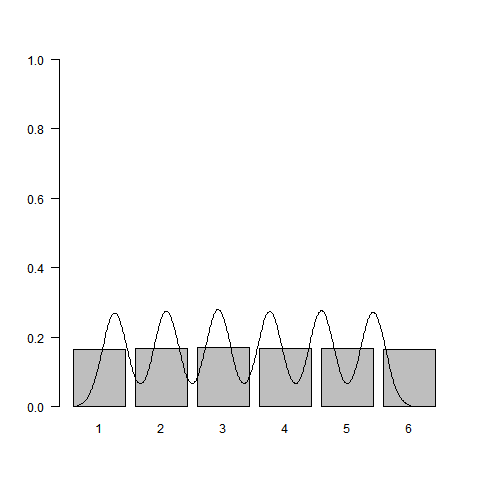
\includegraphics[width=0.3\textwidth]{Files/Images/clm1.png}
    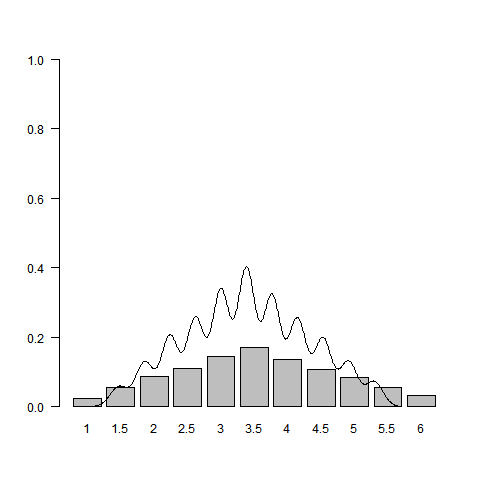
\includegraphics[width=0.3\textwidth]{Files/Images/clm2.png}
    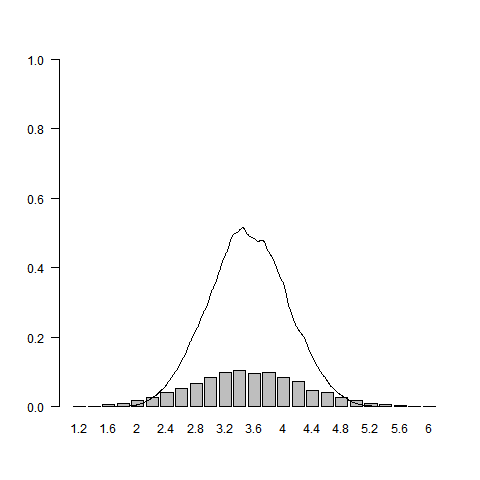
\includegraphics[width=0.3\textwidth]{Files/Images/clm5.png} \\
    \rcode{dice = 1} \hspace{3.3cm} \rcode{dice = 2} \hspace{3.3cm} \rcode{dice = 5}
\end{center}

Saying that the sample distribution becomes more tight around 3.5 as a result of increasing the sample size (the number of \rcode{dice}) can be expressed in a mathematical way:

\begin{equation*}
    \sigma_{\text{sampling distribution}} = \frac{\sigma_{\text{population}}}{\sqrt{n}},
\end{equation*}

where $\sigma$ is the \concept{standard deviation} and $n$ is the size of your sample. So if the sample size is very large, you can expect the \concept{standard deviation} of the \concept{sampling distribution} to be rather small. Important is that the \concept{mean} of the \concept{sampling distribution} is the same as the \concept{population mean}, but the \concept{standard deviation} is not. 

\clearpage % Page break